\section{神经网络--前向算法}

\subsection{神经网络示意图--前向算法}
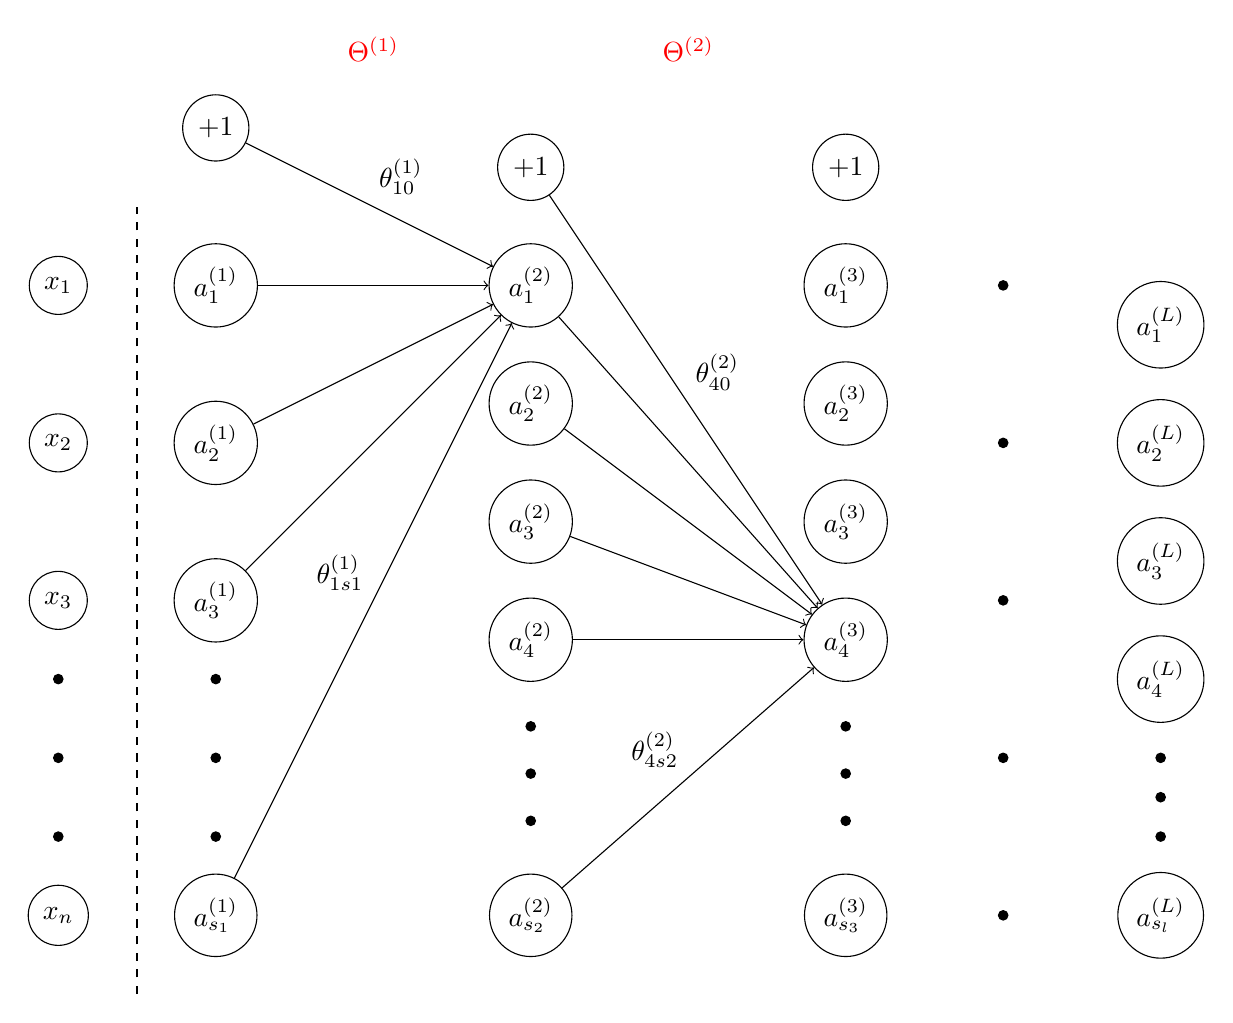
\begin{tikzpicture}
\tikzset{
	a/.style={circle, draw=black}
}

% x
% \node[a] (x_0) at(0,10) {$x_0=+1$};
\node[a] (x_1) at(0,8) {$x_1$};
\node[a] (x_2) at(0,6) {$x_2$};
\node[a] (x_3) at(0,4) {$x_3$};
\filldraw (0,3) circle (.06);
\filldraw (0,2) circle (.06);
\filldraw (0,1) circle (.06);
\node[a] (x_n) at(0,0) {$x_n$};

% X与a的分隔线
\draw [dashed] (1,-1) -- (1,9);

% a^{(1)}
\node[a] (a_10) at(2,10)   {$+1$};
\node[a] (a_11) at(2,8)   {$a_1^{(1)}$};
\node[a] (a_12) at(2,6) {$a_2^{(1)}$};
\node[a] (a_13) at(2,4)   {$a_3^{(1)}$};
\filldraw (2,3) circle (.06);
\filldraw (2,2) circle (.06);
\filldraw (2,1) circle (.06);
\node[a] (a_1s1) at(2,0) {$a_{s_1}^{(1)}$};

% a^{(2)}
\node[a] (a_20) at(6,9.5) {$+1$};
\node[a] (a_21) at(6,8.0) {$a_1^{(2)}$};
\node[a] (a_22) at(6,6.5) {$a_2^{(2)}$};
\node[a] (a_23) at(6,5.0) {$a_3^{(2)}$};
\node[a] (a_24) at(6,3.5) {$a_4^{(2)}$};
\filldraw (6,2.4) circle (.06);
\filldraw (6,1.8) circle (.06);
\filldraw (6,1.2) circle (.06);
\node[a] (a_2s2) at(6,0) {$a_{s_2}^{(2)}$};

% a^{(3)}
\node[a] (a_30) at(10,9.5) {$+1$};
\node[a] (a_31) at(10,8.0) {$a_1^{(3)}$};
\node[a] (a_32) at(10,6.5) {$a_2^{(3)}$};
\node[a] (a_33) at(10,5.0) {$a_3^{(3)}$};
\node[a] (a_34) at(10,3.5) {$a_4^{(3)}$};
\filldraw (10,2.4) circle (.06);
\filldraw (10,1.8) circle (.06);
\filldraw (10,1.2) circle (.06);
\node[a] (a_3s3) at(10,0) {$a_{s_3}^{(3)}$};

% 中间部分
\filldraw (12,0) circle (.06);
\filldraw (12,2) circle (.06);
\filldraw (12,4) circle (.06);
\filldraw (12,6) circle (.06);
\filldraw (12,8) circle (.06);

% a^{(n)}

\node[a] (a_L1) at(14,7.5) {$a_1^{(L)}$};
\node[a] (a_L2) at(14,6)   {$a_2^{(L)}$};
\node[a] (a_L3) at(14,4.5) {$a_3^{(L)}$};
\node[a] (a_L4) at(14,3)   {$a_4^{(L)}$};
\filldraw (14,2.0) circle (.06);
\filldraw (14,1.5) circle (.06);
\filldraw (14,1.0) circle (.06);
\node[a] (a_Lsl) at(14,0) {$a_{s_l}^{(L)}$};


% 前向算法图例--仅连线:a1 -- a_21
% \draw[->] (a_10) -- (a_21);
\draw[->] (a_11) -- (a_21);
\draw[->] (a_12) -- (a_21);
\draw[->] (a_13) -- (a_21);
% \draw[->] (a_1s1) -- (a_21);

% 前向算法图例--有标注:a1 -- a_21
\path (a_10) edge[->] node[auto] {$\theta_{10}^{(1)}$} (a_21);
% \path (a_11) edge[->] node[auto] {$\theta_{11}^{(1)}$} (a_21);
% \path (a_12) edge[->] node[auto] {$\theta_{12}^{(1)}$} (a_21);
% \path (a_13) edge[->] node[auto] {$\theta_{13}^{(1)}$} (a_21);
\path (a_1s1) edge[->] node[auto] {$\theta_{1s1}^{(1)}$} (a_21);


% 前向算法--仅连线: a2 --> a34
% \draw[->] (a_20) -- (a_34);
\draw[->] (a_21) -- (a_34);
\draw[->] (a_22) -- (a_34);
\draw[->] (a_23) -- (a_34);
\draw[->] (a_24) -- (a_34);
% \draw[->] (a_2s2) -- (a_34);

% 前后算法图例--有标注:a2 -- a34
\path (a_20) edge[->] node[auto] {$\theta_{40}^{(2)}$} (a_34);
% \path (a_21) edge[->] node[auto] {$\theta_{41}^{(2)}$} (a_34);
% \path (a_22) edge[->] node[auto] {$\theta_{42}^{(2)}$} (a_34);
% \path (a_23) edge[->] node[auto] {$\theta_{43}^{(2)}$} (a_34);
% \path (a_24) edge[->] node[auto] {$\theta_{44}^{(2)}$} (a_34);
\path (a_2s2) edge[->] node[auto] {$\theta_{4s2}^{(2)}$} (a_34);


% 下方的标志
\node at (4, 11) {\color{red}{$\Theta^{(1)}$}};
\node at (8, 11) {\color{red}{$\Theta^{(2)}$}};

\end{tikzpicture}


\begin{equation}
	a^{(j)} = g(z^{(j-1)}) \Rightarrow {(m,s_j)}
\end{equation}

\begin{equation}
	\Theta^{(j)} = 
		\left(\begin{matrix}
			\theta_{10}^{(j)} & \theta_{11}^{(j)} & \theta_{12}^{(j)} & \dots & \theta_{1,s_{j}}^{(j)} \\
			\theta_{20}^{(j)} & \theta_{21}^{(j)} & \theta_{22}^{(j)} & \dots & \theta_{2,s_{j}}^{(j)} \\
			\theta_{30}^{(j)} & \theta_{31}^{(j)} & \theta_{32}^{(j)} & \dots & \theta_{3,s_{j}}^{(j)} \\
			\vdots    & \vdots    & \vdots    & \ddots & \vdots   \\
			\theta_{s_{j+1}0}^{(j)} & \theta_{s_{j+1}1}^{(j)} & \theta_{s_{j+1}2}^{(j)} & \dots & \theta_{s_{j+1},s_{j}}^{(j)}
		\end{matrix}\right) \Rightarrow {(s_{j+1},s_{j}+1)}
\end{equation}

\begin{equation}\begin{aligned}
	z^{(j+1)} &= (1, a^{(j)}) (\Theta^{(j)})^T \\
		\\ &= 
			\left(\begin{matrix}
				z_1^{(j+1)(1)} & z_2^{(j+1)(1)} & z_3^{(j+1)(1)} & \dots & z_{s_{j+1}}^{(j+1)(1)} \\
				z_1^{(j+1)(2)} & z_2^{(j+1)(2)} & z_3^{(j+1)(2)} & \dots & z_{s_{j+1}}^{(j+1)(2)} \\
				z_1^{(j+1)(3)} & z_2^{(j+1)(3)} & z_3^{(j+1)(3)} & \dots & z_{s_{j+1}}^{(j+1)(3)} \\
				\vdots & \vdots & \vdots & \ddots & \vdots \\
				z_1^{(j+1)(m)} & z_2^{(j+1)(m)} & z_3^{(j+1)(m)} & \dots & z_{s_{j+1}}^{(j+1)(m)} \\
			\end{matrix}\right)
\end{aligned}\end{equation}

\begin{equation}
	a^{(j+1)} = g(z^{(j+1)})  \Rightarrow {(m,s_{j+1})} 
\end{equation}


\begin{equation} \begin{aligned}
	y & = \left(\begin{matrix}
			y^{(1)} \\ y^{(2)} \\ y^{(3)} \\ \vdots \\ y^{(m)} \\
		\end{matrix}\right)_{m*1}
\end{aligned} \end{equation}
